% UTF-8

% single-chapter commands
\documentclass{../thesis} \setcounter{chapter}{1} \begin{document}


\chapter{Analyse der Ausgangslage}

\section{OpenStreetMap: Alles für Alle}
Topographische Vermessungen führten ursprünglich nur zu relativ ungenauen Ergebnissen \cf[43]{Koh04}. Für die im 18.~und 19.~Jahrhundert erstmals durchgeführte systematische Landesaufnahme standen nur am Boden operierte Messinstrumente zur Verfügung. Bis in die zweite Hälfte des 20. Jahrhunderts waren der manuell horizontierte und abgelesene Theodolit und das Bandmaß die dabei primär eingesetzten Instrumente \cf[3–6]{WG06}. Deren Natur entsprechend ging dies mit einem immensen Aufwand an Arbeitskräften einher.

Die schiere Menge der eingesetzten Vermesser machte im Laufe der Zeit auch mit einfachen Instrumenten zufriedenstellende Ergebnisse möglich. In den letzten Jahrzehnten haben Photogrammetrie, Fernerkundung und satellitengestützte Ortsbestimmung das Vermessungswesen revolutioniert. Genauere Resultate ließen sich in kürzerer Zeit und so auch mit geringeren Kosten erreichen. \noref

% Ist die Kostendiskussion wirklich von Interesse? Eigentlich geht's ja nur um die ursprüngliche Motivation für OSM

Obgleich die Kosten geringer als zuvor sind, liegen sie nach wie vor in mehrstelliger Millionenhöhe allein für die amtlichen Geobasisdaten eines deutschen Bundeslandes \cf[3]{lgm05}.
% [lgm05 3 (LG München, Beschl. vom 9. Nov. 2005, Az. 21 O 7402/02, 3; in: GRUR 2006, 225)]
In Europa \noref herrscht heutzutage \cf[119]{Fis01} die Auffassung vor, dass diese solcherart mit Steuergeldern erhobenen Daten der Allgemeinheit nicht kostfrei zur Weiternutzung zur Verfügung gestellt werden, sondern die \emph{konkreten} Nutzenden zusätzlich Lizenzgebühren zahlen sollen \noref. Diese Lizenzkosten schränken den Nutzen amtlicher Geodaten nicht nur für kommerzielle Zwecke \cf[336]{Böh07}, sondern auch für Privatleute \noref erheblich ein \noref.

% [Egg99 \noref]

Heute haben selbst billige GPS-Empfänger eine Genauigkeit, welche die mancher Vermessung des 19. Jahrhunderts übertreffen kann \cf[346][\?]{WG06}. Die „freie Weltkarte“ \eyecatcher{OpenStreetMap} (OSM) \cf[3]{RT09} macht sich dies zu Nutze, um mit Hilfe zehntausender Freiwilliger eine weltweite Datenbank mit Geobasisdaten aufzubauen und nachzuführen (Volunteered Geographic Information, VGI) \cf[147, 154]{NZ12}. Im Gegensatz zu vielen amtlichen Geobasisdaten dürfen OpenStreetMap-Daten lizenzkostenfrei verwendet werden, auch für kommerzielle Zwecke \cf[217, 221\f]{RT09}.

% ODBL? -> 3rd ed

% fühlt sich alles _viel_ zu lang an … was davon brauche ich wirklich als Überleitung zu Fragmentierung und Process?
% straff kürzen, unbekannte Begriffe a la KV-Pair einfach in Fußnote packen…
% Oder wild ausdehnen, z. B. Verweis auf NoSQL-Prinzip hinsichtlich Flexibilität? … Nein, das ist nicht Aufagbe dieser Arbeit. Lieber noch mehr Verweise suchen.

Der Name OpenStreetMap mag fehlleitend sein, denn es handelt sich dabei nicht um eine Straßenkarte, sondern vielmehr um eine Geodatenbank mit Inhalten nahezu beliebiger Themen. Bei der Gründung von OSM im Jahr 2004 wurde auf das Festlegen starrer Klassifizierungsschemata oder Kartierschlüssel verzichtet. Statt dessen kann jedes Element in der Datenbank mit einer beliebigen Anzahl Attribute – sogenannter \term{tags} – versehen werden, die jeweils aus einem Schlüssel und einem Wert bestehen \term{(key-value-pair)}. \cf[56]{RT09}

% ways / relationen / fragmentierung !!

Syntax und Semantik der einzelnen \term{tags} werden bei OpenStreetMap seit der Gründung fortlaufend von den Beitragenden diskutiert, gestützt auf bisherige Erfahrungen. Die Diskussion findet vornehmlich im Internet statt; Ergebnisse werden öffentlich dokumentiert und in Software wie z.~B. Renderern implementiert. Wer neue Inhalte erfasst, orientiert sich oft an den bisher in der Datenbank üblichen oder im Web dokumentierten Konventionen. \cf[48]{Top09} \cf[17\f, 59–66]{RT09}

Gegenüber einer vor der Erfassung vereinbarten gemeinsamen Ontologie \cf[14]{GOS09} hat dieses System zur Folge, dass die zu OSM Beitragenden genau das erfassen, was sie persönlich interessiert und für wichtig halten. Jeder der Beitragenden entscheidet die Kriterien für die Erfassungsgeneralisierung für sich selbst. %Dies führt zu großen regionalen Unterschieden in Datendichte, -aktualität und -qualität.
% Regionalität ist nicht entscheidend für uns.

% Verweis auf Sch09 deckt schon vieles ab; Kne09 eher knapp, Beh11 noch knapper, Kla11 umständlich

Oft verfügen die OpenStreetMap-Daten über sehr hohen Detailreichtum. So könnten zum Beispiel für Teilstücke einer Straße \term{tags} für Tempolimits, Überholverbote, Fahrspurenanzahl, Oberflächenmaterial sowie -Qualität, Baujahr und mehr eingetragen worden sein. Veränderungen an diesen Attributen im Verlauf der Straße führen im OSM-Datenmodell zwangsläufig zu einer Fragmentierung in mehrere aufeinander folgende Linienabschnitte \term{(ways)}, jeweils mit unterschiedlichen \term{tags} \cf[57]{RT09}.

% "Detailreichtum entsprechend einer Grundkarte" (?) -> verdeutlicht, dass OSM ungeneralisiert ist

Baulich getrennte Fahrbahnen wie etwa Autobahnen bildet OpenStreetMap mittels zweier paralleler Einbahn-Linienzüge ab \cf[62]{RT09}. Dies ist eine in der Geoinformatik gängige Vorgehensweise \cf[2][\?]{Tho05}.

Sowohl die Fragmentierung als auch die parallelen Linienzüge führen zu Schwierigkeiten in der Weiterverarbeitung und Visualisierung \noref[Mig12 u. a.].
% Abbildungen:
% - Marker-Wucherung
% - stark unregelmäßige Plazierung von Namen \cf{Mig12}
% - Blitzer/Freistellung
% - Doppelnamen \cf{Mig12}
% o. ä.
Offensichtlich ist, dass eine Verkettung der Fragmente bzw. parallelen Linienzüge als Bestandteil des Datenmodells die Probleme wesentlich verkleinern, wenn nicht gar gänzlich lösen würde. Für eine hierarchisch orientierte Organisation wie etwa Vermessungsämter wäre eine solche Lösung naheliegend. Über \term{relations} ist dies auch in OpenStreetMap möglich \cf[57]{RT09}. Das oben beschriebene Fehlen interner Strukturen unter den zu OpenStreetMap Beitragenden (der \term{community}) macht es jedoch unmöglich, „mal eben“ die Regeln für die Erfassung und Kodierung der Geodaten zu ändern \cf{Sch09}.

% unklar: "hierarchisch orientierte Organisation"? gemeint ist wohl das Ding mit der manuell gepflegten Mittellinie in den Daten?

Statt dessen müssen Änderungsvorschläge erst von der \term{community} akzeptiert und anschließend \emph{großräumig} und \emph{korrekt} in der Datenbank Anwendung finden. Die Erfahrung zeigt, dass dies ein langwieriger Prozess sein kann, der umso schwieriger wird, je geringer der unmittelbare Einfluss der Datenbank-Änderungen auf das in Karten sichtbare Ergebnis ist \noref.


% OSM ist per design völlig ungeneralisiert, da maßstabslos und für auch sehr große maßstäbe eingesetzt. WIrd das im Zusammenhang deutlich? wichtig für logik im folgeabschnitt



%\biggap

\section{Kartenherstellung mit OpenStreetMap} \label{kartenherstellung}

Wohl am bekanntesten ist OpenStreetMap für die auf der Projekt-Homepage \url{osm.org} zugängliche Web-Karte (Abbildung~\ref{fig:osm.org}).
% Erkläung zu "wohl" in Fußnote übertrieben, da Zusammenhang trivial; siehe Mail Dietmar.
Sie besteht aus quadratischen Kacheln \term{(tiles)} von $256\times\unit[256]{px}$, die dort in 20 verschiedenen Maßstäben angeboten werden von etwa $1 \colon 2000$ bis $1 \colon 500~\unit{Mio.}$ \cf[154–155]{RT09}
% http://wiki.openstreetmap.org/wiki/Zoom_levels <-- ersetzt RT09 154f, ist auch aktueller; RT09 hat nur 19 zoomlevel!
Eine interaktive Oberfläche erlaubt über die freie Wahl der \term{Zoomstufe} eine Maßstabswahl und macht den Kartenausschnitt verschiebbar, so dass jeder im eingesetzten Kartennetz abbildbare Punkt der Erde angezeigt werden kann.
\noref %evtl. irgendwas aus RT09 für Kachelanzahl im größten Maßstab}
% evtl. Datenmenge etc. betonen

% Zoomstufe deutsch? -> alles im Duden checken! Konsistenz ist für \term entscheidend -DGD

\begin{figure}[ht]
    \centering
    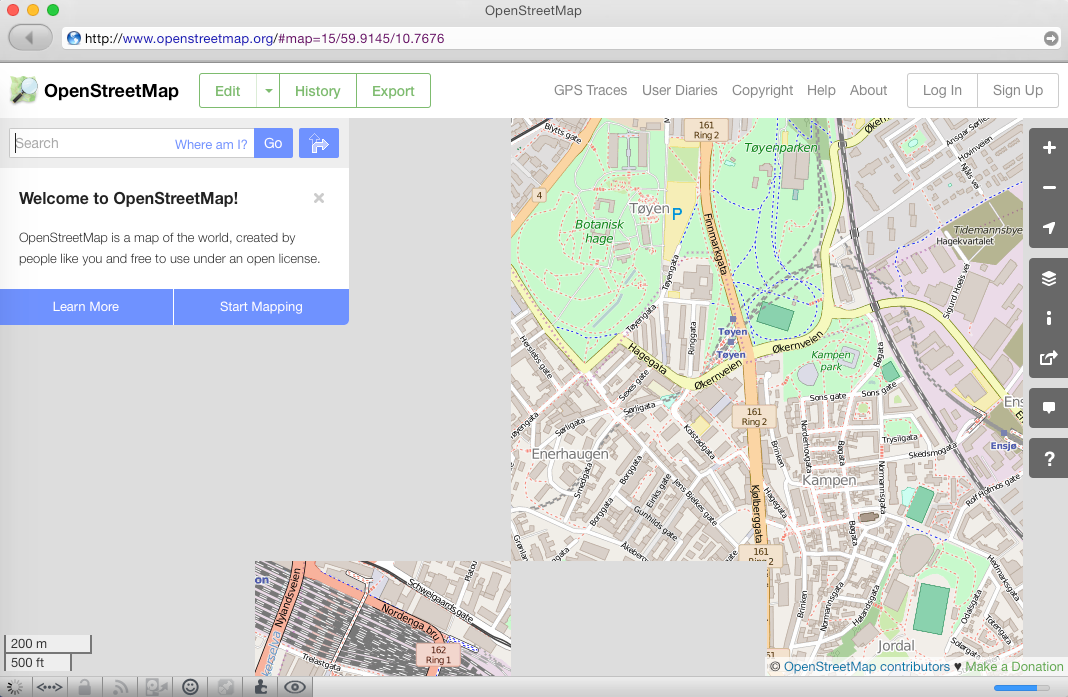
\includegraphics[width=\ScaleIfNeeded]{../chapter2/osm-org}
    \caption{Projekt-Homepage von OpenStreetMap während des Ladevorgangs}\label{fig:osm.org}
\end{figure}

Wegen der sehr großen Anzahl von Kacheln werden diese in größeren Maßstäben \term{just in time} gezeichnet. Die Kartenbasis ist für alle Maßstäbe die jeweils minutengenau aktualisierte OSM-Datenbank. \noref % evtl. Verweis auf RT09, insb. für basis, minutengenau -> p. 157 zu osmarender, -> p. 195 zu diffs
% just in time: http://wiki.openstreetmap.org/wiki/Mod_tile

Diese schnelle Aktualisierung ist für OpenStreetMap besonders wichtig, um den freiwillig Mitwirkenden nach einem Beitrag zur Datenbank ein schnelles Erfolgserlebnis zu geben, indem der Beitrag in der Karte weltweit für jeden sofort sichtbar wird.
Aus diesem Grund muss jede Generalisierung der Karte automatisiert ablaufen. Weiterhin bedeutet die Zahl der Beiträge mit teilweise über 1000 \term{changesets} pro Stunde, \cf{osm15}
% http://osmstats.neis-one.org/?item=changesets&date=7-11-2015
% http://neis-one.org/2013/08/osm-activity-report-2013/
dass der Arbeitsaufwand für eine manuelle Generalisierung prohibitiv hoch wäre. Klassische kartographische Generalisierung von Hand kommt daher nur für nicht nachzuführende und geographisch begrenzte Einzelanfertigungen in Betracht, etwa wenn auf Basis von OpenStreetMap eine traditionelle gedruckte Karte hergestellt werden soll.

Typischerweise besteht die Grundlage für Web-Karten wie derjenigen auf \url{osm.org} aus einer Geodatenbank, die mit einer Kopie der OpenStreetMap-Datenbank gefüllt und anschließend minütlich aktualisiert wird. Diese Geodatenbank enthält die Geometrie und Attribute der Rohdaten. Vom Kartenleser in der interaktiven Oberfläche im Webbrowser erzeugte Anfragen nach Kacheln der Karte werden dann von der Renderer-Software unter Zugriff auf die Geodatenbank abgearbeitet, wobei die Geometrie anhand der vorgegebenen Zeichenregeln dargestellt wird. Gerenderte Kacheln werden gecacht und zum Browser geschickt.

Eigene Bearbeitungsschritte zur Generalisierung von Daten sind bei diesem Ablauf nicht vorgesehen (im Gegensatz zu den Abläufen im AAA-Modell der deutschen Landesvermessung \cf[263, KN 62 (5)]{ML12}). Lediglich als Nebeneffekt des Einlesens in die Datenbank und des Zeichnens durch den Renderer wird eine begrenzte Modell-\noncf[194 17.2]{RT09} bzw. kartographische Generalisierung durchgeführt. \cf[194, 198]{RT09}
% [ML12] beschreibt einzelne kommerzielle Lösung (hat aber nette Bilder); -> möglichst noch bessere Quelle suchen
% http://wiki.openstreetmap.org/wiki/Mod_tile/Setup_of_your_own_tile_server

% Skizze OSM-Datenfluss

\begin{figure}[ht]
    \centering
    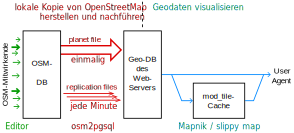
\includegraphics[width=\ScaleIfNeeded]{../chapter2/osm-datenfluss}
    \caption{OSM-Datenfluss}\label{fig:osm-datenfluss}
\end{figure}

% mapnik nur ein beispiel


% obiges trifft auf Linien, Punkte, Flächen gleichermaßen zu; hier darauf eingehen?


% LVAs verwenden (?) kartographische Hints, um die Ableitung von FOlge-DLMs zu erleichtern (?) [ML12, KN 62 (5) 263]. Das geht bei OSM nicht, weil auch das eben die Generalisierung und damti auch die Kartenherstellung verzögern und somit das schnelle ERfolgserlebnis verhindern würde. Es muss eben tatsächlich vollautomatisch ablaufen, wie auch immer.

% lesen: -> KN 56 (4) 191ff Modellgeneralisierung in ATKIS


%\begin{itemize}
%	\item erklären, wie die OSM-Rendering-Pipeline funktioniert, denn zum Verständnis von 2.3 ist wichtig, dass der Renderer die Geometrie nicht ändern kann
%\end{itemize}

% MapCSS includes an eval function, and has rules that act as 'commands' to modify data. CartoCSS does not support eval or any data-modifying operations.
% https://gist.github.com/tmcw/4319642


%\begin{itemize}
%	\item bisher im Wesentlichen nur automatische, (fast) ungeneralisierte Mercator-Tiles fürs Web
%	\item Datenmenge, Maßstäbe, ständige Änderungen und Aktualisierungen etc.
%	\begin{itemize}
%		\item manuelle Generalisierung ist nicht zielführend außer für nicht nachzuführende Einzelanfertigungen
%	\end{itemize}
%	\item in der Praxis fast nur einfache semantische Modellgeneralisierung unmittelbar im Tile-Renderer, keine kartographische Generalisierung oder Folgekarten bzw. -datenbanken
%	\begin{itemize}
%		\item nahe beieinander liegende Punktsignaturen werden willkürlich selektiert, Linearsignaturen überdecken einander
%	\end{itemize}
%	\item insbesondere kaum Vereinfachung, Qualitätsumschlag, Zusammenfassung oder Verdrängung (jedoch einige lohnenswerte Ansätze, z. B. \cf{MWG12} oder Haltestellen-Relationen {z. B. Konrad-Adenauer-Platz Beuel})
%\end{itemize}

% Angesichts dessen wären automatisiert abgeleitete, generalisierte Datenbanken für kleinere Maßstäbe zur Weiterverwendung wünschenswert, existieren jedoch bisher nicht. Entsprechend sind auch die aus OSM-Daten hergestellten Karten in aller Regel nicht kartographisch generalisiert: Nahe beieinander liegende Objekte überdecken einander scheinbar wahllos, Mindestgrößen und notwendige Formvereinfachungen werden von den automatischen Renderern ignoriert.

% Erschwert wird die Generalisierung von OSM-Daten unter anderem durch den hohen Grad der Fragmentierung von Linienzügen. Das Verknüpfen solcher zusammengehörenden, einzelnen ways durch Relationen in der Datenbank ist technisch möglich, wird aber von den Mitwirkenden aus unterschiedlichen Gründen nur sehr selten durchgeführt. Eine automatisierte Generalisierung durch Formvereinfachung (zur Reduktion der node-Anzahl) bedingt daher, dass die zusammengehörenden ways  dabei  als solche identifiziert werden. Gleiches gilt für die Generalisierung durch Zusammenfassung oder Verdrängung parallel verlaufender Linienzüge, beispielsweise Straßen mit begleitendem Radweg oder mehrgleisigen Bahnstrecken.



\section{Automatisierte Linien-Generalisierung von OpenStreetMap-Daten}

Wie im Folgenden einige Beispiele zeigen, lassen sich Auswahl auf Basis der Objektklasse sowie Betonung und Vergrößerung durch veränderte Strichbreite vergleichsweise einfach im Renderer implementieren, da die Geometrie der zugrundeliegenden Geodaten dabei unverändert bleibt. Andere Arten kartographischer Generalisierung wie etwa die Formvereinfachung oder der Qualitätsumschlag verändern die Geometrie und sind damit schwieriger zu implementieren.

\subsection{Generalisierung durch Objektauswahl}

Zur Herstellung der Kacheln der Web-Karte wird notwendigerweise für jede \term{Zoomstufe} eine Auswahl der jeweils  darzustellenden Objektklassen vorgenommen. Beispielsweise werden Anliegerstraßen \term{(residentials)} unterhalb von \term{zoom}~12 nicht mehr dargestellt (Abbildungen~\ref{fig:kampen11} und~\ref{fig:kampen12}). Dies vereinfacht das Kartenbild für den Betrachter und verringert die zu berechnende Datenmenge für den Renderer.

% Qualitätsumschlag fällt in OSM tlws. auch hierunter, gibt's aber nur für Flächen

% screenshots residentials z12 + z11

\begin{figure}[ht]
  \begin{minipage}{.5\linewidth}
    \centering
    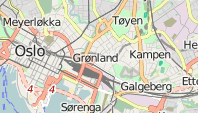
\includegraphics[width=\ScaleIfNeeded]{../chapter2/kampen-z12}
    \caption{Oslo, \term{zoom} 12}\label{fig:kampen12}
  \end{minipage}%
  \begin{minipage}{.5\linewidth}
    \centering
    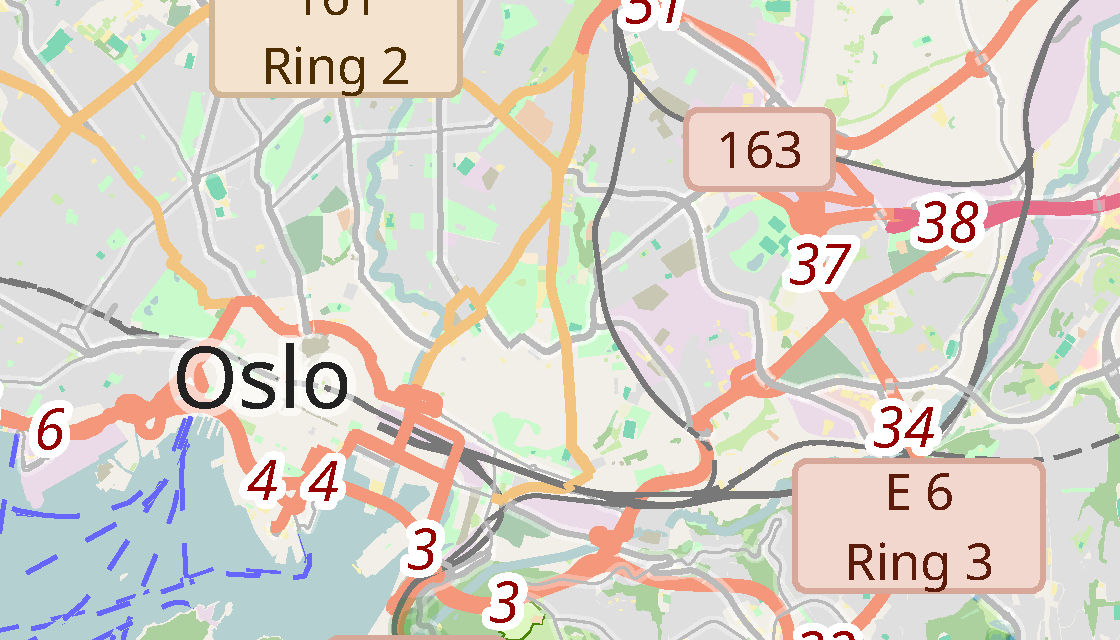
\includegraphics[width=\ScaleIfNeeded]{../chapter2/kampen-z11}
    \caption{Oslo, \term{zoom} 11}\label{fig:kampen11}
  \end{minipage}
\end{figure}




%\begin{figure}[ht]
%  \begin{minipage}{.5\linewidth}
%    \centering
%%    \rule{4cm}{3cm}
%    \includegraphics[width=\ScaleIfNeeded]{../chapter2/test}
%    \caption{Ein Rechteck akudbf sku fbskf bsd fdfb d f,df b dsz bf,ds f,sdzbg sb, fgs fgxh gxh gh}\label{fig:rechteck1}
%  \end{minipage}%
%  \begin{minipage}{.5\linewidth}
%    \centering
%    \captionaboveof{table}
%    [Maße des Rechtecks aus Abbildung~\ref{fig:rechteck1}]%
%    {Maße des Rechtecks}
%    \label{tab:rechteck1}
%    \begin{tabular}{ll}
%      Breite: & 4\,cm\\
%      Höhe: & 3\,cm
%    \end{tabular}
%  \end{minipage}
%\end{figure}

%\includegraphics[width=\ScaleIfNeeded]{../chapter2/test}




\subsection{Generalisierung durch Bewertung}


Weiterhin wird durch die Wahl der Zeichenregeln eine Bewertung der tatsächlich dargestellten Objekte vorgenommen, auch dies abhängig vom Maßstab. So werden Anliegerstraßen auf \term{zoom}~12 als schmaler, einfacher Strich gezeichnet, ab \term{zoom}~13 jedoch als weißer Breitstrich mit grauem Rand (Abbildungen~\ref{fig:kampen12} und~\ref{fig:kampen13}).

% Ist dies Bewertung? Sicherstellen in HGM02 o. ä.
% Hake, Grünreich, Meng 2002 Kartographie (8)

% screenshots residentials z14 + z13

\begin{figure}[ht]
  \begin{minipage}{.5\linewidth}
    \centering
    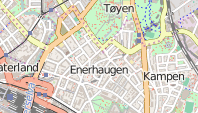
\includegraphics[width=\ScaleIfNeeded]{../chapter2/kampen-z13}
    \caption{Oslo, \term{zoom} 13}\label{fig:kampen13}
  \end{minipage}%
  \begin{minipage}{.5\linewidth}
    \centering
    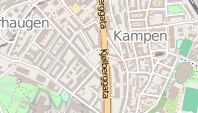
\includegraphics[width=\ScaleIfNeeded]{../chapter2/kampen-z14}
    \caption{Oslo, \term{zoom} 14}\label{fig:kampen14}
  \end{minipage}
\end{figure}


\subsection{Generalisierung durch Vergrößerung}

Die Wahl der Zeichenregeln beinhaltet für einige Objektklassen auch eine Generalisierung durch Vergrößerung, indem für bestimmte Maßstäbe eine Strichbreite gewählt wird, welche im Abbildungsmaßstab die tatsächliche Größe des Objekts übersteigt. Anliegerstraßen haben für die \term{Zoomstufen} 14 bis 19 jeweils eine unterschiedliche Strichbreite von $\unit[3]{px}$ bis $\unit[17]{px}$ definiert, so dass die Darstellung der Straße in der Karte Maßstabsänderungen andeutungsweise folgt (Abbildungen~\ref{fig:kampen17} und~\ref{fig:kampen14}). Die Breite von $\unit[3]{px}$ auf \term{zoom} 14 entspräche ca.~$\unit[27]{m}$ in der Realität \cf[155]{RT09}. Auf \term{zoom} 13 werden Anliegerstraßen gar auf dieselbe Breite von $\unit[3]{px}$ gezeichnet (ca.~$\unit[57]{m}$) und damit deutlich vergrößert, um die Erkennbarkeit im kleinerem Maßstab zu fördern (Abbildungen~\ref{fig:kampen14} und~\ref{fig:kampen13}).

% screenshots residentials z19 o. ä. + CartoCSS/MapCSS-mockup:
% https://github.com/gravitystorm/openstreetmap-carto/blob/fe4f8d48757cf85bb692129b5d9755ba5cadbbee/roads.mss
%@residential-width-z13:           3;
%@residential-width-z14:           3;
%@residential-width-z15:           5;
%@residential-width-z16:           6;
%@residential-width-z17:          12;
%@residential-width-z18:          14;
%@residential-width-z19:          21;

\begin{figure}[ht]
    \centering
    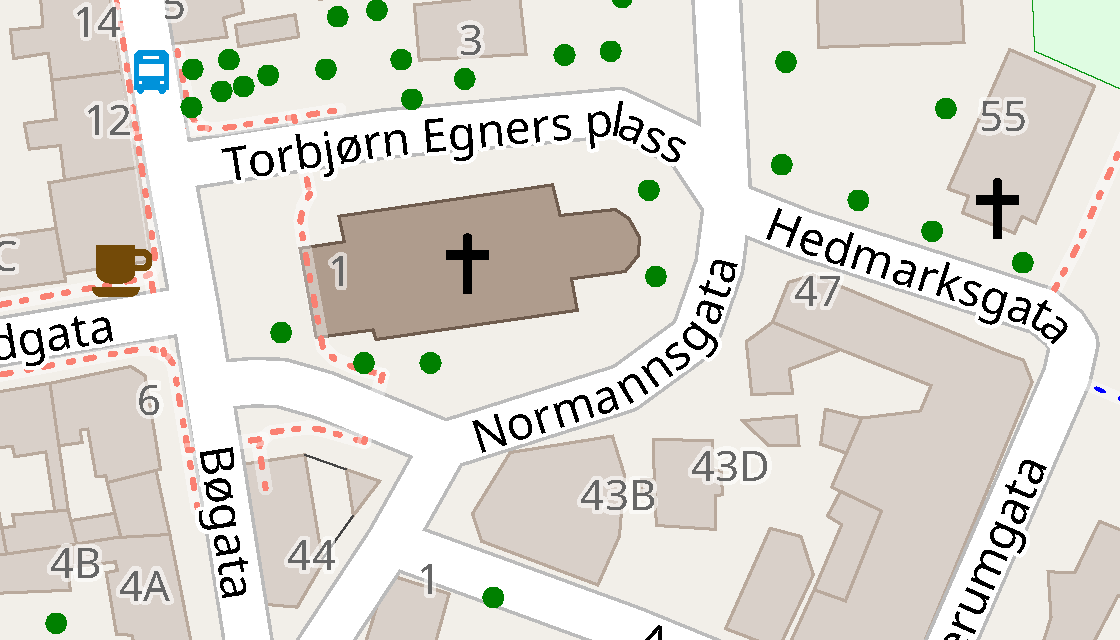
\includegraphics[width=\ScaleIfNeeded]{../chapter2/kampen-z17}
    \caption{Oslo, \term{zoom} 17}\label{fig:kampen17}
\end{figure}

\subsection{Generalisierung durch Formvereinfachung}

% grafik zur fragmentierung?
% grafik zum flussbett?

Eine kartographische Formvereinfachung wird für die Web-Karte nicht vorgenommen. Zufriedenstellende voll automatisiert arbeitende Algorithmen dafür stehen nicht zur Verfügung und ein Eingreifen von Hand ist wie zuvor in Abschnitt \ref{kartenherstellung} erläutert nicht vorgesehen.
% zB Trollstigen - Screenshots auch mit Vergleich zu Kartverket! http://arne.johannessen.de/osm/geocode-adapter/kartverket/?lat=62.459954&lon=7.6703534&zoom=15&layers=B
% zB Lahntalbahn http://www.openstreetmap.org/#map=7/51/8
% "kartographische Formvereinfachung" erklären?

Um die Kosten der Verarbeitung zu senken, ist für geometrische Daten oftmals eine Verringerung der Anzahl der Stützpunkte von Linien wünschenswert. Dies betrifft auch \osm. Entsprechende Algorithmen wie etwa Ramer-Douglas-Peucker [\noref DP73, zt. n. HS92] berücksichtigen jedoch oftmals nur die einzelne Linie unter Vernachlässigung der Netztopologie (Abbildungen~\ref{fig:kardemomme} und~\ref{fig:bab3}).

\begin{figure}[ht]
  \begin{minipage}{.5\linewidth}
    \centering
    \includegraphics[width=\ScaleIfNeeded]{../chapter2/kardemomme}
    \caption{Topologieverlust}\label{fig:kardemomme}
  \end{minipage}%
  \begin{minipage}{.5\linewidth}
    \centering
    \includegraphics[width=\ScaleIfNeeded]{../chapter2/bab3-a}
    \caption{Überkreuzen paralleler Linienzüge}\label{fig:bab3}
  \end{minipage}
\end{figure}

Ein weiteres Hindernis stellt die Fragmentierung der \osm-Linien dar. Bevor etwa über den Ramer-Douglas-Peucker eine nennenswerte Verringerung der \term{node}-Anzahl erreicht werden kann, müssen zunächst die einzelnen \term{ways} entlang des zu vereinfachenden Linienzugs miteinander verknüpft werden.

%Im Übrigen führt eine Verringerung der Zahl der Stützpunkte nicht notwendigerweise zu einer gelungenen kartographischen Generalisierung. Beispielsweise hatten Douglas und Peucker das Ziel \noref{Spekulation}, anhand eines mathematischen Verfahrens die Datenverarbeitung zu vereinfachen, während der sichtbare Linienverlauf nur so wenig wie möglich verändert werden sollte. Von einer Generalisierung nach dem kartographischen Gesichtspunkt „Signifikantes und Repräsentatives bewahren“ ist das Ergebnis regelmäßig weit entfernt. \noref

\begin{itemize}
%	\item Problem bei Formvereinfachung: Fragmentierung sowie Erhalten der geometrischen Topologie
	\item Beispiel: Fluss außerhalb des (unabhängig gemappten) Flussbetts \cf[57]{Kla11}
		\item ebenso bei als Flächen gemappten Straßen oder bei landuse=railway
	\item Beispiel: ungleichmäßiger Abstand (teils sogar negativ, d. h. Überkreuzen) paralleler Fahrbahnen oder Gleise (Skizze oder Screenshot)

	\item zumindest letzteres Beispiel ist lösbar durch vorhergehendes Zusammenfassen
	
	\item Aus diesen Gründen ist Formvereinfachung in kartographisch relevantem Ausmaß nur bei ganzheitlichem Ansatz sinnvoll, der alle Objektklassen berücksichtigt und sie zueinander passend generalisiert. Beispielsweise müsste der Verlauf einer in einem engen Flusstal verlaufenden Straße in gleicher Weise vereinfacht werden wie der Verlauf des Flusses. Wenn nötig, müsste eines dieser beiden Objekte dazu auch verdrängt werden. \cf[90][\? evtl.]{skg02} Ein derart aufwändiger Vorgang wird nicht von dem für die Web-Karte genutzten Renderer Mapnik implementiert. Es wäre ein separater vorgeschalteter Schritt notwendig, welcher aus der lokalen ungeneralisierten Geodatenbank eine separate generalisierte Geodatenbank erzeugt, die dann von Mapnik gerendert werden könnte. Dies ist derzeit nicht der Fall.
\end{itemize}


\subsection{Generalisierung durch Verdrängung}

Typisch für Web-Karten ist das völlige Fehlen von Verdrängungen zur Einhaltung kartographischer Minimalabstände und -dimensionen. Statt dessen werden mit kleiner werdendem Maßstab Objekte dichter und dichter aneinander, schließlich gar übereinander gezeichnet, worunter das Kartenbild teils erheblich leidet (Abbildung~\ref{fig:verdraengung}). Web-Karten mit \osm-Daten sind hier keine Ausnahme.

\begin{figure}[ht]
    \centering
    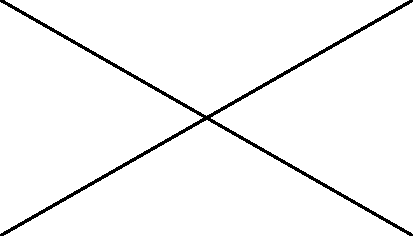
\includegraphics[width=\ScaleIfNeeded]{../image-missing}
    \caption{Typisches Generalisierungsergebnis in Web-Karten; fiktives Beispiel nach [sgk02, 49]}\label{fig:verdraengung}
\end{figure}

% Bevor eine Generalisierung durch Verdrängung stattfinden kann, muss zunächst der ohne Verdrängung entstehende Konflikt [das Hindernis] erkannt werden.
% Skizze zur Erläuterung (?)


\subsection{Generalisierung durch Zusammenfassung}

\begin{itemize}
%	\item hier: ohne Flächen zu berücksichtigen, obwohl dort evtl. ähnliche Probleme auftreten könnten
% (ich glaube, ähnliche Probleme treten eigentlich nicht auf)
	
%	\item Auswahl, Vergrößern und Betonen funktioniert zufriedenstellend
%		\item einfache Screenshots aus osm.org als Beispiele
	
	\item Problem bei Zusammenfassung: Linienzüge müssen (oft?) als zusammengehörig (z. B. parallel) erkannt werden, bevor zusammengefasst werden kann
	
	% Qualitätsumschlag? railway=rail -> landuse=railway ?
	
\end{itemize}


\section{Zielsetzung der Arbeit}

Im Falle paralleler Linienzüge treten immer wieder in verschiedenen Situationen Darstellungsprobleme auf. Beispielsweise variiert in OpenStreetMap auffallend oft der Abstand von zwei Richtungsfahrbahnen einer Straße. Abbildung~\ref{fig:b256} zeigt, wie innerhalb weniger hundert Meter die Linearsignaturen zweier Richtungsfahrbahnen teilweise so weit voneinander entfernt liegen, dass dazwischen eine Lücke entsteht, aber teilweise auch so dicht beieinander, dass die Lücke geschlossen wird und die Randstriche der beiden Signaturen ineinander übergehen, was den Eindruck eines Mittelstriches wechselnder Strichstärke erwirkt. An einer Stelle sind die beiden Richtungsfahrbahnen gar so dicht beieinander gezeichnet, dass der Rand- bzw. Mittelstrich verschwindet und beide Fahrbahnen ineinander übergehen.

\begin{figure}[ht]
  \begin{minipage}{.5\linewidth}
    \centering
    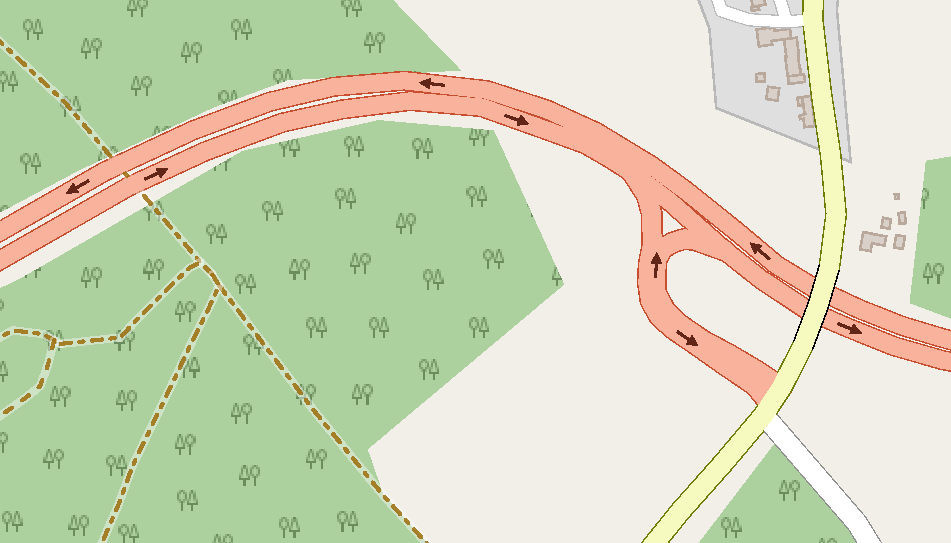
\includegraphics[width=\ScaleIfNeeded]{b256@2-z16}
    \caption{variierende Abstände von Richtungsfahrbahnen, B\,256n (50~\%, bearbeitet)}\label{fig:b256}
  \end{minipage}%
  \begin{minipage}{.5\linewidth}
    \centering
    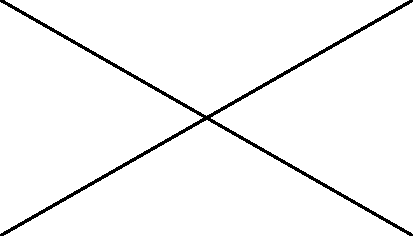
\includegraphics[width=\ScaleIfNeeded]{../image-missing}
    \caption{kombinierte Signatur für autobahnähnliche Straße}\label{fig:dual-carriageway}
  \end{minipage}
\end{figure}

In Maßstabsbereichen, in denen die Grundrisstreue keine Rolle spielt, könnte möglicherweise eine statt dessen mittig zwischen den beiden Fahrbahnen gezeichnete kombinierte Signatur ein besseres Kartenbild erreichen (Abbildung~\ref{fig:dual-carriageway}). Da jedoch in \osm{} eine gesonderte Erfassung einer Mittellinie als Straßenachse unüblich ist, müssten hierzu zunächst die beiden Richtungsfahrbahnen als zusammengehörig (parallel) erkannt werden.

% 256 (großer maßstab)
% dual carriageway (kleiner maßstab) (evtl. fotos trunk NO)

In Deutschland erfasst die \osm-\term{community} autobahnähnliche Straßen als \tag{highway=trunk} aufgrund ihres Ausbauzustands. \noref[wiki DE] Allerdings bildet die \osm-Straßenklassifizierung historisch bedingt das britische System ab, wo \term{trunk roads} ausdrücklich keinen bestimmten Ausbauzustand haben, sondern das Kernnetz der wichtigsten Straßen erster Ordnung bilden. \noref[wiki EN] Unter Umständen wird \tag{highway=trunk} somit auch für schmalere Landstraßen verwendet. Gleiches gilt u.~a. für Norwegen (\term{riksveg}, Abbildung~\ref{fig:trunk-norway}).

% TODO: schauen, ob Karte von Dolkviktunnelen / Rv557 besser passt, weil beide Richtungen des Problems gezeigt werden (analog rail tracks) -- theoretisch ja, aber vmtl. schwierig umzusetzen

% TODO: Relationen-Probleme erläutern? -> eher weiter vorne!

% Ev39 Kalandseidet, > 6 m aber Karte zeigt "mitten im Dorf"
% Ev39 Søfteland, Bild noch besser, aber keine Häuser in Karte
% Ev39 nach Nesttun rein, ginge auch, aber mit Radweg
%   https://goo.gl/maps/jYRgZVXft912
% Ev39 Vallaheiene wohl das beste hier
%   https://goo.gl/maps/wMHPCocqsSH2
% Rv13 Låtefossen, würde auch ohne Häuser in Karte funktionieren, < 6 m
% oder so Serpentinen, z. B. Granvin, gutes Bild aber keine Bebauung in Karte
%   https://goo.gl/maps/Y4NwWfRWSZ82

%\begin{figure}[ht]
%  \begin{minipage}{.5\linewidth}
%    \centering
%    \includegraphics[width=\ScaleIfNeeded]{trunk-no-rv13-photo}
%    \caption{ein \tag{highway=trunk} im ländlichen Norwegen (Rv13, Låtefossen)}\label{fig:trunk-norway}
%  \end{minipage}%
%  \begin{minipage}{.5\linewidth}
%    \centering
%    \includegraphics[width=\ScaleIfNeeded]{trunk-no-rv13-map1}
%    \caption{Die für \tag{highway=trunk} gewählte Signatur lässt in Norwegen zum Teil einen weit besseren Ausbauzustand vermuten als vorhanden.}\label{fig:trunk-norway-osm-de}
%  \end{minipage}
%\end{figure}

\begin{figure}[ht]
  \begin{minipage}{.5\linewidth}
    \centering
    \includegraphics[width=\ScaleIfNeeded]{trunk-no-ev39-photo2}
    \caption{typischer \tag{highway=trunk} in Norwegen (E\,39, Vallaheiane)}\label{fig:trunk-norway}
  \end{minipage}%
  \begin{minipage}{.5\linewidth}
    \centering
    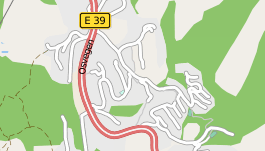
\includegraphics[width=\ScaleIfNeeded]{trunk-no-ev39-map1}
    \caption{Die hier für \tag{highway=trunk} gewählte Signatur lässt einen weit besseren Ausbauzustand vermuten als in Norwegen zum Teil vorhanden (Vallaheiane).}\label{fig:trunk-norway-osm-de}
  \end{minipage}
\end{figure}

%\begin{figure}[ht]
%  \begin{minipage}{.5\linewidth}
%    \centering
%    \includegraphics[width=\ScaleIfNeeded]{trunk-no-serp-photo}
%    \caption{ein \tag{highway=trunk} im ländlichen Norwegen (ehem. Rv13, Skjervet)}\label{fig:trunk-norway}
%  \end{minipage}%
%  \begin{minipage}{.5\linewidth}
%    \centering
%    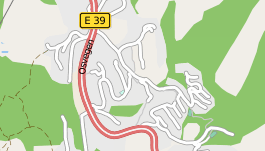
\includegraphics[width=\ScaleIfNeeded]{trunk-no-ev39-map1}
%    \caption{Die für \tag{highway=trunk} gewählte Signatur lässt in Norwegen zum Teil einen weit besseren Ausbauzustand vermuten als vorhanden.}\label{fig:trunk-norway-osm-de}
%  \end{minipage}
%\end{figure}

Wird den Gepflogenheiten in Deutschland entsprechend für \tag{highway=trunk} eine auf einen Ausbau mit baulich getrennten Fahrbahnen hindeutende Signatur gewählt, so birgt dies im internationalen Einsatz Potenzial für Verwirrung (Abbildung~\ref{fig:trunk-norway-osm-de}). Dass aus dem \osm-Datenmodell samt Attributen der tatsächliche Straßenzustand oft nicht hervorgeht, macht die Möglichkeit einer algorithmischen Ableitung aus der Geometrie der Geodaten interessant.
% Möchte man einheitliche Zeichenregeln verwenden, so wäre auch hier eine Erkennung als zusammengehörig hilfreich.

Ein unklares Kartenbild ist jedoch auch in weniger exotischen
% "näher liegenden"?
Konstellationen zu beobachten. Ein weit verbreitetes Problem ist beispielsweise eine scheinbare Variation der Breite von auf \url{osm.org} gezeichneten Straßen. Abbildung~\ref{fig:utrecht14} zeigt, wie die als Sammelstraße klassifizierte Croeselaan mit breiterem Strich gezeichnet wird als Teile der Hauptstraßen. Grund dafür sind nicht tatsächliche Unterschiede im Ausbauzustand, sondern der Umstand, dass die Fahrbahnen der niederrangigen Straße durch einen breiten, parkähnlichen Grünstreifen getrennt werden  (Abbildung~\ref{fig:utrecht16}). In kleinerem Maßstab überlappen sich die Striche der beiden Fahrbahnen und fließen zusammen. Ebenfalls auffallend ist in Abbildung~\ref{fig:utrecht14} die wechselhafte Strichbreite der links im Bild von Nordwest nach Süd verlaufenden Hauptstraße.

% gera/utrecht - evtl. MapQuest / osm.de hier einbringen
\begin{figure}[ht]
  \begin{minipage}{.5\linewidth}
    \centering
    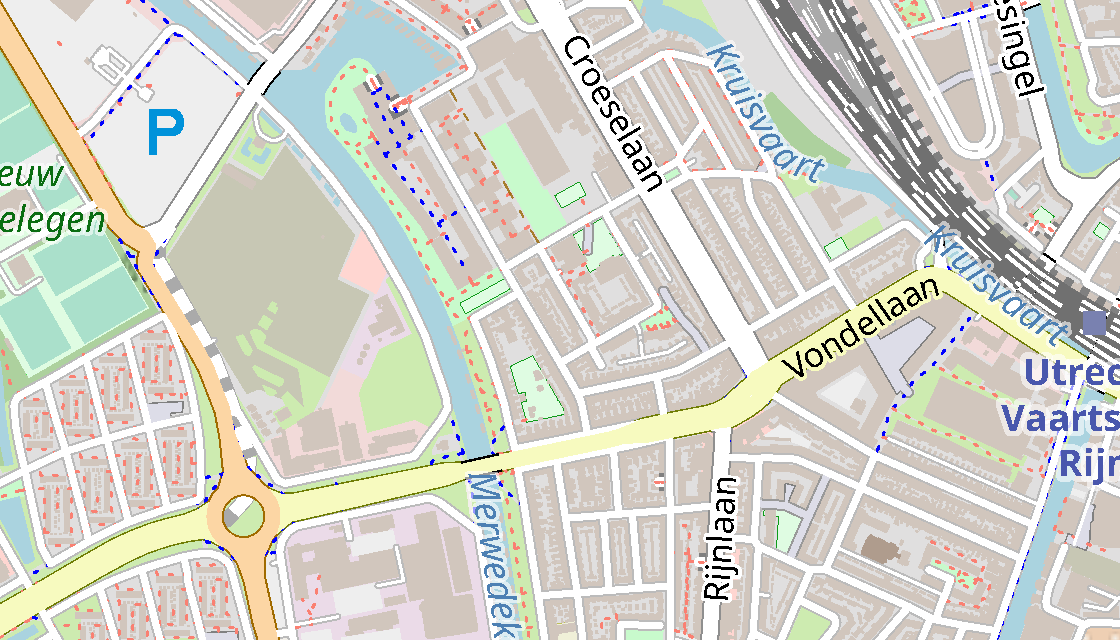
\includegraphics[width=\ScaleIfNeeded]{utrecht-z14}
    \caption{Utrecht, \term{zoom} 14}\label{fig:utrecht14}
  \end{minipage}%
  \begin{minipage}{.5\linewidth}
    \centering
    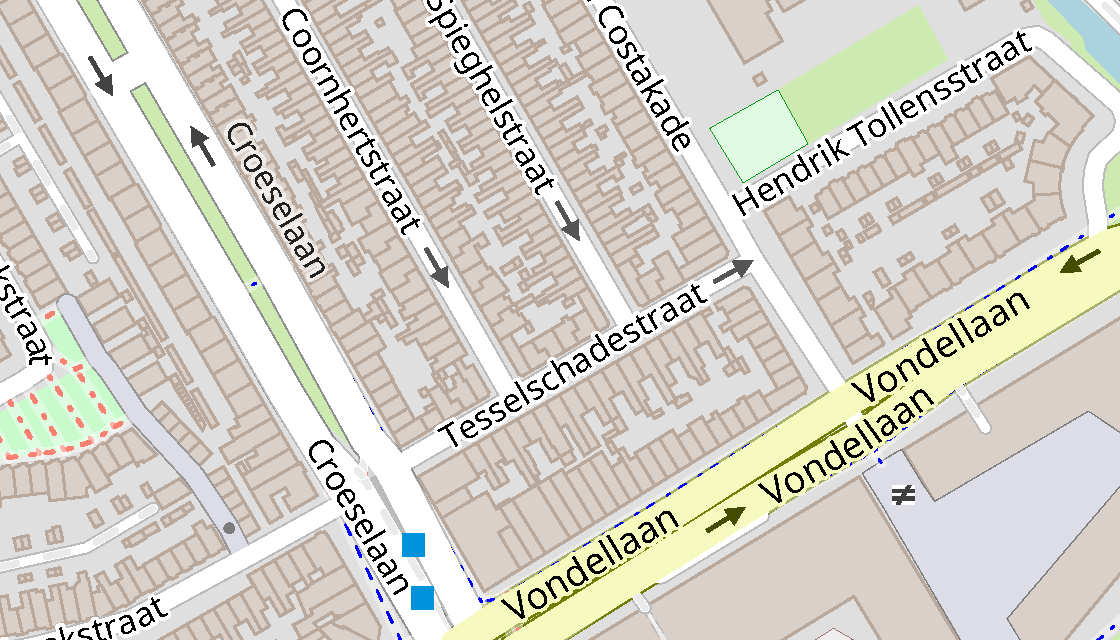
\includegraphics[width=\ScaleIfNeeded]{utrecht-z16}
    \caption{Utrecht, \term{zoom} 16}\label{fig:utrecht16}
  \end{minipage}
\end{figure}

% zweite Abbildung mit überlagerten Ways?

Abbildung~\ref{fig:gera13} zeigt ähnliche Probleme. Die Strichbreite der aus Südosten in die Stadt Gera hineinführenden Hauptstraße ist in deren Verlauf nicht konstant, sondern wechselt scheinbar unmotiviert. Dann nach Norden zwischen Fluss und Eisenbahn wird dieselbe Straße erheblich breiter, ab der Kreuzung nach Westen am Ortsteil Debschwitz vorbei auf einmal wieder schmaler.

% Absatz etwas unklar, insb. letzter Satz (implizit)
Würde man den Maßstab stark vergrößern, träte an diesen Stellen die gleiche Ursache zutage wie oben anhand Abbildung~\ref{fig:b256}
%und~\ref{fig:utrecht16}
gezeigt: Die Straßen verfügen über baulich getrennte Richtungsfahrbahnen und werden deshalb mit zwei Linienzügen in der Datenbank modelliert, deren Abstände variieren. Die bauliche Trennung ist überdies nicht überall vorhanden.

\begin{figure}[ht]
  \begin{minipage}{.5\linewidth}
    \centering
    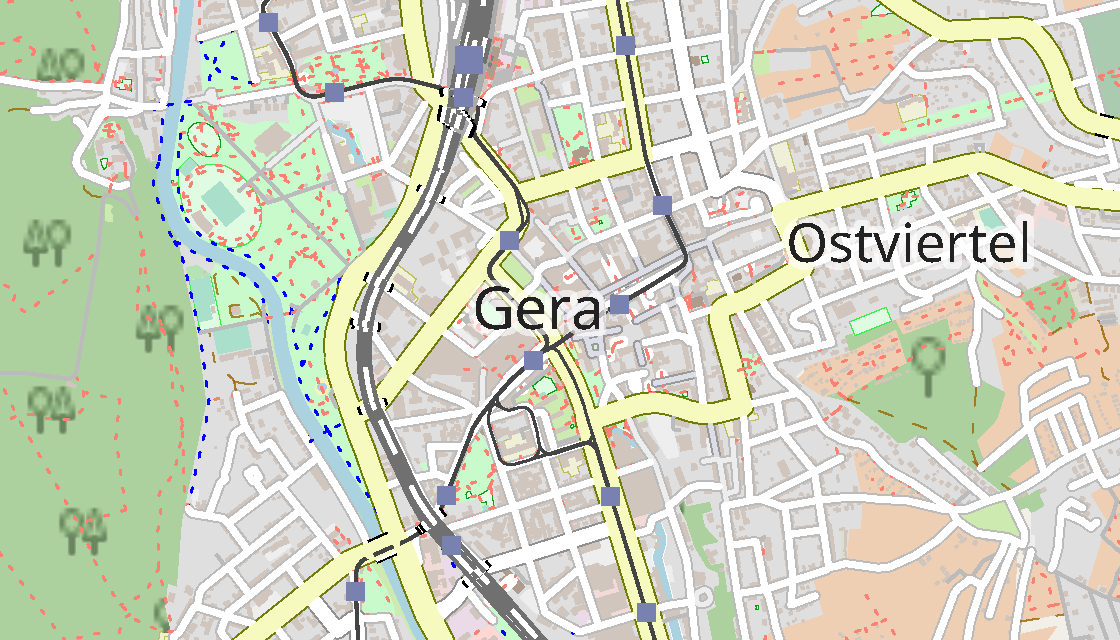
\includegraphics[width=\ScaleIfNeeded]{gera-z13}
    \caption{Gera, \term{zoom} 13}\label{fig:gera13}
  \end{minipage}%
  \begin{minipage}{.5\linewidth}
    \centering
    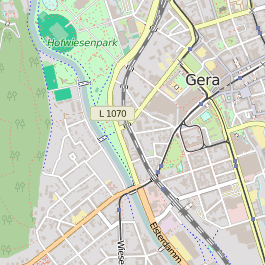
\includegraphics[width=\ScaleIfNeeded]{gera-z14}
    \caption{Gera, \term{zoom} 14}\label{fig:gera14}
  \end{minipage}
\end{figure}

In Gera ergibt sich besonders im Vergleich zweier Maßstäbe ein unklares Kartenbild. Westlich des Zentrums verläuft eine Hauptstraße in einem Abschnitt sehr dicht neben der Bahnstrecke. In großem Maßstab (Abbildung~\ref{fig:gera14}) scheint die Straße an dieser Stelle breiter zu sein als ein paar Meter weiter südlich, wo der Abstand zur Bahnstrecke größer ist. In kleinem Maßstab (Abbildung~\ref{fig:gera13}) erscheint dieses Verhältnis umgekehrt. Dies liegt daran, dass die Straße in genau diesem Abschnitt baulich getrennte Fahrbahnen hat, in kleinerem Maßstab aber teilweise durch die Bahnstrecke verdeckt wird. 

Solcherart einander verdeckende Linien sind ebenfalls verbreitet. Abbildungen~\ref{fig:stuelinghausen-mapnik} und~\ref{fig:stuelinghausen-maps.me} zeigen, wie ein straßenbegleitender Radweg mal „über“, mal „unter“ der Straße zu liegen kommt. Keiner dieser beiden Ansätze ist kartographisch gelungen. Zu lösen wäre dieser Konflikt durch eine Generalisierung durch Verdrängung (siehe weiter unten).

% stülinghausen/verdrängung
\begin{figure}[ht]
  \begin{minipage}{.5\linewidth}
    \centering
    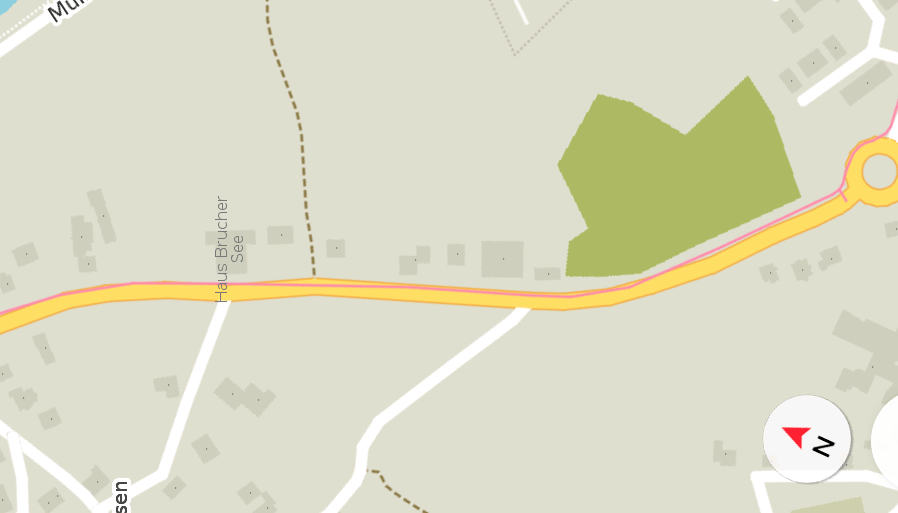
\includegraphics[width=\ScaleIfNeeded]{stuelinghausen-me}
    \caption{stuelinghausen-me}\label{fig:stuelinghausen-maps.me}
  \end{minipage}%
  \begin{minipage}{.5\linewidth}
    \centering
    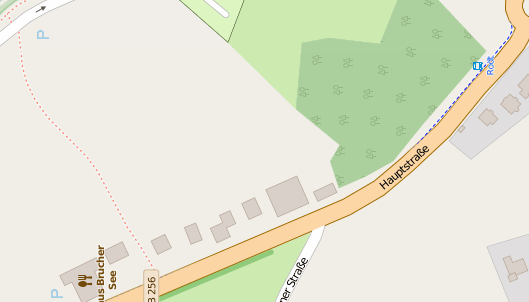
\includegraphics[width=\ScaleIfNeeded]{stuelinghausen@2-z17}
    \caption{stuelinghausen@2-z17}\label{fig:stuelinghausen-mapnik}
  \end{minipage}
\end{figure}

% zu tracks=* - Überleitung evtl:
% Folge der oben beschriebenen offenen Arbeitsweise von \osm ist, dass das Herstellen einer Einigung über bestimmte Tagging-Varianten und deren Anwendung durch die Community oft ein langsamer Prozess ist. \noref[Sch09, forum 485926 s.u.]

Die Probleme sind nicht auf das Straßennetz beschränkt. Mit \tag{tracks=*} wird in \osm{} die Anzahl der Eisenbahngleise gekennzeichnet, für die ein \term{way} steht. Abbildungen~\ref{fig:tracks-small} und~\ref{fig:tracks-large} stellen diesen \term{tag} farblich dar. Bei Betrachtung in kleinem Maßstab (Abbildung~\ref{fig:tracks-small}) sieht (1) zunächst nach einer viergleisigen Strecke aus, in Abbildung~\ref{fig:tracks-large} plötzlich nach einer insgesamt 16gleisigen Strecke. Tatsächlich liegen insgesamt vier einzelne Gleise. Möglicherweise hat ein \osm-Beitragender \tag{tracks=*} missverstanden als die Gesamtanzahl der Gleise [Forum], wofür jedoch ein anderer \term{tag} steht (\tag{passenger\_lines=*}).
% http://lists.openstreetmap.org/pipermail/tagging/2012-August/011066.html

% track
\begin{figure}[ht]
  \begin{minipage}{.5\linewidth}
    \centering
    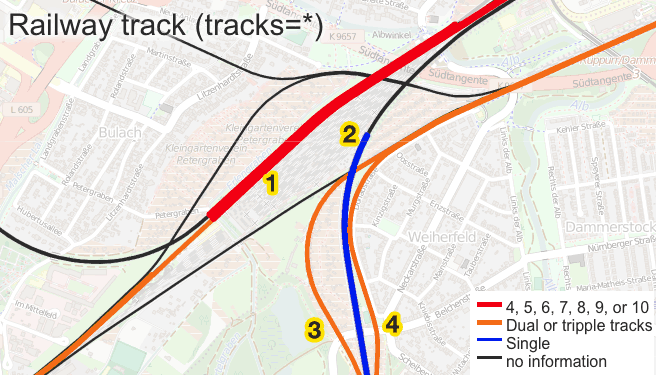
\includegraphics[width=\ScaleIfNeeded]{tracks-small}
    \caption{tracks-small}\label{fig:tracks-small}
  \end{minipage}%
  \begin{minipage}{.5\linewidth}
    \centering
    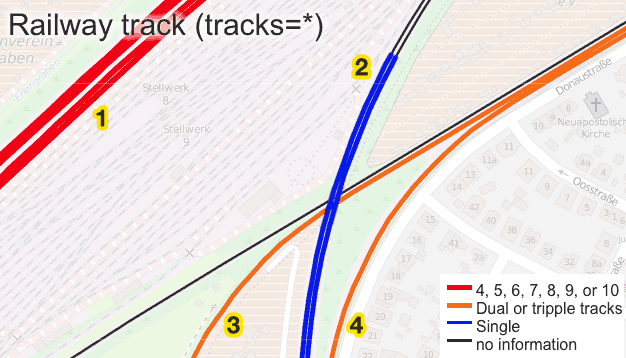
\includegraphics[width=\ScaleIfNeeded]{tracks-large}
    \caption{tracks-large}\label{fig:tracks-large}
  \end{minipage}
\end{figure}

Analog kann in Abbildung~\ref{fig:tracks-small} der Eindruck entstehen, dass von der eingleisigen Strecke (2) zwei doppelgleisige Strecken (3) und (4) derart abzweigen, dass am unteren Bildrand insgesamt fünf Gleise nebeneinander liegen. In größerem Maßstab (Abbildung~\ref{fig:tracks-large}) wird (2) plötzlich der Realität entsprechend als zwei parallele Gleise erkennbar, deren Signaturen im kleineren Maßstab zusammengeflossen waren. Der Abzweig (3) und (4) besteht tatsächlich aus jeweils einem einzelnen Gleis, das fälschlich \tag{tracks=2} gesetzt hat.

% Fußnote?
Insgesamt ist diese Karte mit \tag{tracks=*} wenig gelungen. Hier zeigt sich eine Schwäche von \osm: Zwar ist mit \term{relations} eine logische Verknüpfung paralleler Gleise in der \osm-Datenbank technisch möglich, jedoch ist dies nicht zuverlässig und simpel genug, dass es von einer Mehrheit der \osm-Beitragenden angewandt wird. Das unglücklich benannte \tag{passenger\_lines} reicht für manche Anwendungen aus, wird jedoch nur auf speziellen Karten angezeigt,
% zu implizit?
so dass es nicht annähernd flächendeckend erfasst ist (Abbildung~\ref{fig:passenger_lines}).

\begin{figure}[ht]
  \begin{minipage}{.5\linewidth}
    \centering
    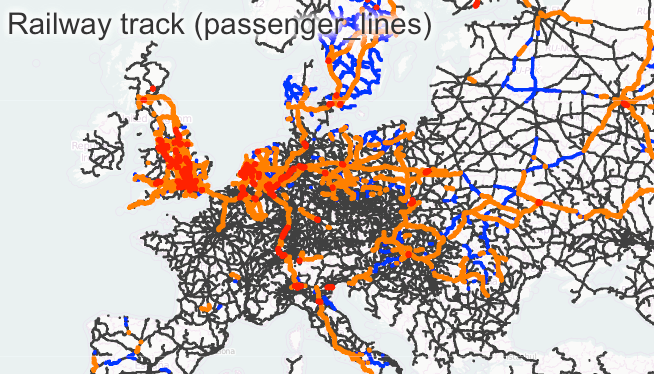
\includegraphics[width=\ScaleIfNeeded]{passenger_lines-europe}
    \caption{passenger-lines}\label{fig:passenger_lines}
  \end{minipage}%
  \begin{minipage}{.5\linewidth}
    % überkreuzen
    \centering
    \includegraphics[width=\ScaleIfNeeded]{bab3-a}
    \caption{Überkreuzen paralleler Linienzüge}\label{fig:bab3}
    % evtl. neue Screenshots aus QGIS o.ä. anfertigen?
  \end{minipage}
\end{figure}

% mit heißer Nadel geschrieben...
Optisch besonders auffällig ist fehlende Erkennung paralleler Linienzüge als zusammengehörig, wenn sie einer starken Formvereinfachung unterzogen werden. Weil beide Linien dann unabhängig voneinander generalisiert werden, kann es abhängig vom eingesetzten Algorithmus zu unterschiedlichen Formen der beiden Linien kommen, die sich im Extremfall sogar gegenseitig überkreuzen können (Abbildung~\ref{fig:bab3}).
% (kurzer Verweis auf vorgenannte Probleme)

%\item Erkennung als parallel ist bisher ein Problem
% [CTGV14] benennen?
% _war_ bisher! oder "ist gewesen"...

%\textbf{offener Punkt: Redundanz mit Themenblatt}

% (die Beispiele wiederholen sich => bessere Abgrenzung der Kapitel)

% -> Google Traffic
% nur hier nennen...? -> bessere Kapitelabgrenzung!

% google
%\begin{figure}[ht]
%    \centering
%    \includegraphics[width=\ScaleIfNeeded]{google-traffic}
%    \caption{google-traffic}\label{fig:google-traffic}
%\end{figure}

%%%%%%%%%%%%%%%%%%%%%%%%%%%%%%%%%%%%%%%%%%%%%%%%%%%%%%%%%%%%%%
%%%%%%%%%%%%%%%%%%%%%%%%%%%%%%%%%%%%%%%%%%%%%%%%%%%%%%%%%%%%%%
% \eyecatcher{Ziel der Arbeit}
% im Prinzip sollte NUR dieser Unterabschnitt in Kapitel 2.4 stehen, alles hierüber sollte in 2.3 (das jedenfalls war das ursprüngliche Konzept)!
% Mal sehen, ob das noch aktuell ist ... 2.4 würde dann ja SEHR kurz(?).
%%%%%%%%%%%%%%%%%%%%%%%%%%%%%%%%%%%%%%%%%%%%%%%%%%%%%%%%%%%%%%
%%%%%%%%%%%%%%%%%%%%%%%%%%%%%%%%%%%%%%%%%%%%%%%%%%%%%%%%%%%%%%


\section{(2.4) Zielsetzung der Arbeit}

Das automatisierte Zusammenfassen paralleler Linienzüge kann zur Vermeidung einiger der oben diskutierten Probleme bei der Generalisierung und Darstellung von Geodaten beitragen.

Bereits das Zusammenfassen selbst ist ein Vorgang der kartographischen Generalisierung. Es kann das Kartenbild vereinfachen und verbessern.
% TODO: Abgleich mit oben

Beim Zusammenfassen können Attribute der beteiligten \term{ways} derart aggregiert werden, dass zuvor durch Geometrie ausgedrückte Zusammenhänge in den generalisierten Daten erhalten bleiben. Beispielsweise kann beim Zusammenfassen paralleler Gleise die in \tag{passenger\_lines} vermerkte Gleisanzahl der zuvor getrennten \term{ways} für das generalisierte Ergebnis addiert werden. Die so vereinfachten Geodaten können dann entsprechend ihrer Attribute visualisiert werden. Die Gefahr von missverständlichen oder unschönen Kartenbildern, die wie oben gezeigt etwa durch Überlagerung entstehen können, wird so verringert.

Ebenfalls verringert wird die Datenmenge an sich. Das Arbeiten mit Geodaten für große Gebiete, aber auch die Weiternutzung für andere Zwecke wird so unter Umständen einfacher.
% (möglichst Zahlenbeispiele für Dateigröße, Featurezahl und/oder Laufzeiten anhand meiner Skripte für größere OSM-Datensätze nennen)

Zum Beispiel sind automatisierte Formvereinfachungen einfacher durchzuführen, wenn keine Rücksicht auf parallele Linienzüge mehr genommen werden muss (siehe Beispiel oben mit überkreuzenden Linien).
% TODO: Referenz
% Zusammenfassung kann theoretisch auch Erstellen von MRDBs vereinfachen

Ziel \emph{dieser} Arbeit ist die Entwicklung von Algorithmen zur Generalisierung durch Zusammenfassung parallel verlaufender Linienzüge in \osm{}. Weitere Generalisierungsvorgänge sind nicht Teil dieser Arbeit, insbesondere weder eine Formvereinfachung noch eine Verdrängung.


%\begin{itemize}
%	% „Algorithmen zur automatisierten Generalisierung durch Zusammenfassung von Linienzügen in OpenStreetMap“
%	
%	\item \eyecatcher{Ziel der Arbeit:} die automatisierte Generalisierung durch Zusammenfassung von Linienzügen
%	
%	\item Visionen:
%	\begin{itemize}
%		\item kartographische Generalisierung => besseres Kartenbild
%			\item Zusammenfassung der Attribute derart, dass die Möglichkeit zur Darstellung der Gesamtwerte besteht (z. B. Railway-Tracks / lanes)
%		\item Verringerung der Datenmenge => einfacheres Arbeiten mit Daten für große Gebiete, Vereinfachung der Weiternutzung
%			(möglichst Zahlenbeispiele für Dateigröße, Featurezahl und/oder Laufzeiten anhand meiner Skripte für größere OSM-Datensätze nennen)
%		\item Zusammenfassung kann theoretisch auch Erstellen von MRDBs vereinfachen
%	\end{itemize}
%	
%	\item \emph{nicht} Teil der Arbeit sind insbesondere:
%	\begin{itemize}
%		\item die Formvereinfachung selbst
%		\item eine wie auch immer geartete Verdrängung (obgleich eine solche durch diese Arbeit vielleicht erleichtert werden könnte)
%	\end{itemize}
%\end{itemize}


\section[Diskussion existierender Ansätze]{(2.5) Diskussion existierender Ansätze zur automatisierten Linien-Generalisierung}

\begin{itemize}

	% ! Puffer
	\item Puffer \cf[2–3]{OHSZ10}
% - für eine Darstellung von OSM-Daten als Teil eines 3D-Modells werden Straßen "realistisch" verbreitert per Buffer in PostGIS
% - um Fragmente und Parallelen zu beseitigen, werden die so entstandenen Polygone nun vereinigt
% => Parallelen finden durch Buffer-Algorithmus und Polygonanalyse
% => Epsilon benötigt
% - Buffer orthogonal zur Linie würde reichen; die Endrundungen können wegfallen
% - löst Zusammenfassung nicht, da keine unmittelbare Rückführung zur Linie allein mit diesem Ansatz möglich (was für das erklärte Ziel 3D aber eh nix ausmacht, insofern ist der Ansatz gut, aber eben nicht gut für mich); evtl. inward offset (um wieviel?) oder eher -> Skeleton
% - löst auch Erkennung nicht
	
	% ! Skeleton
	\item Skeleton \cf{LM96} \cf{Mig12} \cf[][\?]{All11}
	% HS04: straight skeleton for MRDB
	% <http://web.archive.org/web/20070613154012/http://www.ikg.uni-hannover.de/skalen/buendel/PDF/Skeleton.pdf>
	% - "In geometry, a straight skeleton is a method of representing a polygon by a topological skeleton." (<- Wikipedia)
	% - Ziel: Framework für MRDB (automatisch)
	% - erwähnt Chordal Axis (Prasad, 1997) ********
	% - verwendet straight skeleton plus eine handvoll Regeln, um Kreuzungen etc. zu behandeln; immer noch etwas verwurstet, aber sieht wesentlich besser/systematischer aus als LM96
	% - schlägt angeblich fehl an komplizierteren Stellen
	% - ermittelt eine Relation zwischen ALK ATKIS
	% Mig12: Projekt für "schöne" topo. Karte
	% <http://mike.teczno.com/notes/osm-us-terrain-layer/foreground.html>
	% <http://mike.teczno.com/img/terrain-stamen-post/>
	% - erwähnt kurz Probleme von dual carriageways
	% - eines der Probleme: unschöne versetzte Doppelungen von Straßennamen
	% - Anwendung von Skeletron (mit Implementierung von LM96 für OSM)
	% - Ziel letztlich "nur" Shields und Straßennamen
	% Skeletron [Mig11/ME11 (?)]:
	% <https://github.com/migurski/Skeletron>
	% - jetzt LM96, davor HS04 (?) "straight skeleton", was nicht so toll war
	% LM96: Straßen_flächen_ -> Einzellinie
	% - Ziel: Eliminierung _oder_ Minimierung manueller Eingriffe
	% - gute Ausgangsdaten seien entscheidend fürs Projekt gewesen (1:1000, mit Straßenflächen!)
	% - ways werden verdichtet auf einen node alle 30 cm, um eine gesmoothte Mittellinie zu erhalten
	% - ausgehend von nodes wird ein Voronoi-Diagramm gebaut, aus dem sich direkt die Mittellinie ergibt (nach filtern)
	% - erzeugt schwierig zu filternde Dangles / Forks dort, wo Parallelen enden; Auflösung durch zusätzliche Angaben aus der Datenquelle ('The "true end" of the road is determined by temporarily appending the appropriate road extent arcs from the original Urban layer.')
	% - "Suspect situations" kommen vor und werden manuell beseitigt
	% - 7 man-months
	%  All11: ????
	
	% ! Strokes
	\item Strokes \cf{Tho06b} \cf{EM00} \cf{TR99}
	% Tho06b: Netzwerk-Generalisierung und -Analyse
	% - perzeptueller Ansatz zur Defragmentierung und Auswahl-Generalisierung
	% - primär Behandlung kollinearer Linien, erwähnt beiläufig aber auch Erkennung von Parallelen [evtl. mehr in den zahlreichen Referenzen darin?]
	% - "perceptual grouping" [684]
	% EM00:
	% - erwähnt sehr deutlich meine Probleme mit "hanging streets" an Kreuzungen etc. [3]
	% - erwähnt keine Parallelen, zeigt aber Implementierung der Theorien von Tho06b bzw. TR99
	
	% ! OS MasterMap
	\item OS MasterMap \cf{CM05}
	% CM05: ganzheitlicher Ansatz für Ordnance Survey in Road Network
	% - arbeitet primär mit Strokes; Problem dabei: "good continuation" sieht an Gabelungen u. U. je nach Seite unterschiedlich aus; zur Lösung werden Attribute herangezogen
	% - Fig 10 zeigt Resultat, welches Parallelen hat, welche nicht erwähnt werden
	% - hebt Kreuzungsproblem als ungelöst hervor
	
	\cf{Tho05}
	% (ähnelt grob meinem Ansatz)
	% Tho05: speziell meine Problemstellung!
	% - Ziel: Hilfe bei automatischer Folgekartenableitung beim Ordnance Survey
	% - 3 wichtigste Teile: Kreuzungsproblem, Verdrängung und Zusammenfassung von Parallelen [2]
	% - arbeitet mit Strokes basierend auf one-way-Attributen; Probleme an manchen Kreuzungen, die aber automatisch erkannt und behoben werden sollen
	% - Paarbildung erfolgt abhängig von Klassifizierung der Strokes (z. B. bei Verkehrsinseln kleinere Höchstschwelle als bei normalen Straßen)
	% - klappt nicht in allen Fällen (einzelne Fehlerfälle)
	% - benutzt Skeleton zur tatsächlichen Zusammenfassung der erkannten Paare
	% - funktioniert meistens, aber nicht immer; manche der Restfälle manuell als nicht lösbar erkannt
	% - one-way-Attribut war "essential"
	% - Ergebnis hat noch keine Topologie (future work)
	% - erst mit Topologie ist Unterbrechung der Signatur möglich, um Ampelkreuzungen im Dual Carriageway darzustellen
	% - Kreisverkehre werden bisher ignoriert
	
	% ! graphbasiert
	\item graphbasiert \cf{JC04} \cf{MM99} \cf{HAS05} \cf{TR95} \cf{Kne09}
	% JC04: connectivity graph für urban street network
	% - dreht Straßen-Graph logisch um (Knoten=Straße, Kante=Verbindung)
	% - filtert nach Graphkriterien ("centralities" degree, closeness, betweenness)
	% - Ergebnis ist ein nach natürlich Kriterien modellgeneralisiertes Netz, denn Straßen mit besserer Verbindung werden häufiger benutzt und sind somit wichtiger
	% - Parallelen im Straßennetz zeichnen sich durch Redundanz und Symmetrie aus (oft gegeneinander gerichtete Einbahnstraßen) und sind damit höchstens! in einem sehr unregelmäßigen Netz theoretisch! erkennbar; tatsächlich werden im Beispiel im Paper die Parallelen nicht generalisiert [168]
	% MM99: Simplification of Junctions
	% - "Brücken von Königsberg" als Beispiel für junction simplification und Zusammenfassung von Parallelen, aber das ist wohl etwas zu sehr vereinfacht! [188]
	% - evtl. werden durch Zusammenfassen der Kreuzung von Parallelen jene zu Duplikaten und können so erkannt und zusammengefasst werden; Nachteil: klappt wirklich nicht ohne Kreuzungen (diese Methode wird anscheinend nicht explizit erwähnt)
	% HAS05: will typische Muster erkennen
	% - erwähnt für Strokes Problem dort, wo Richtungsfahrbahnen beginnen, mitsamt theoretischer Lösung [3.2]
	% - evtl. können Parallelen in einem Netzwerk durch Musteranalyse erkannt werden (typischerweise sehr lang und schmal); jedoch vmtl. Probleme an Kreuzungen etc.
	% TR95: Graphentheorie in der Generalisierung von Straßennetzen
	% - betont, dass autom. Generalisierung oft Darstellungs-zentriert ist und Topologie des Ergebnisses vernachlässigt [1871]
	% Kne09: Anwendung von Graphentheorie in OSM, wenig hilfreich für uns
	% MB93: Graphentheorie in der Generalisierung allgemein
	% - durch Prüfung der Einbahn-Richtung erkennen, ob insgesamt ein verbundener Graph vorliegt (zweimal Einbahn => einmal Zweibahn)
	
	% ! Relational Constraints
	\item Relational Constraints \cf{TBDJRG12}
	% - hat keinen Algorithmus, sondern nur Konzepte
	% - führt constraint ontology ein als mögl. Hilfswerkzeug
	% evtl. als Grundlage für Kap. 4 interessant
	
	% ! Conflict Detection
	\item Conflict Detection \cf{KP98} \cf{Tho06a}
	% KP98:
	% - Ziel: gesamtes Straßennetz
	% - detektiert Fälle, in denen Linien einander zu nahe kommen (wobei Bereiche nahe der Endknoten jeweils ausgeschlossen werden)
	% - nutzt Voronoi region
	% - eigentlich nicht speziell für parallelen gedacht oder geeignet (nutzt Dijkstra, um längeren von zwei Wegen zu eliminieren), aber speziell der "Second step: eliminate conflicts" könnte anwendbar sein, und der Voronoi-Kram gibt zumindest ein paar hübsche Bilder
	% Tho06a: ? Bib, einzelne Fotos in "neu"
	% - erwähnt ausdrücklich mein Problem als "hilfreich" (in gelöstem Zustand)
	% - Skeleton??
	
\end{itemize}

% + RoadMatcher 
% <http://wiki.openstreetmap.org/wiki/Roadmatcher>
% + http://sourceforge.net/projects/jump-pilot/files/OpenJUMP_plugins/More%20Plugins/Matching%20PlugIn/
% <http://sourceforge.net/projects/jump-pilot/files/OpenJUMP_plugins/More%20Plugins/Matching%20PlugIn/>

(jeweils einschließlich Anwendbarkeit auf die vorliegende Fragestellung, ggf. Vor- und Nachteilen, ggf. Bezug der darin verwendeten Fachsprache zur in dieser Arbeit verwendeten Terminologie)



\nocite{*}  % include works in bibliography that aren't cited anywhere in the document (for debugging)

% single-chapter commands
\listoffigures %\listoftables
\bibliographystyle{../myAMSalpha} \bibliography{../thesis}{}
\end{document}
